\documentclass[german,a4paper,12pt,oneside]{paper}
% $Id: notes.tex,v 1.33 2005/03/09 14:16:39 thoss Exp $
\usepackage[scale={0.7,0.8}]{geometry}
\usepackage[english]{babel}   
\usepackage[latin1]{inputenc}   % use the babel multi-languages macros and 
%\usepackage[applemac]{inputenc} %!! For Umlauts!!1!
\usepackage{color}
\usepackage[centertags]{amsmath} 
\usepackage{upref,theorem}
\usepackage{minitoc}
\usepackage{graphicx}
\usepackage{array,cite}
\usepackage{pifont}
\usepackage{type1cm}
\usepackage[psamsfonts]{amssymb}
\usepackage{xspace}
\usepackage{rcs,calc}
\usepackage{pstricks,pst-node}
\usepackage[small,indent]{caption2}
\usepackage{listings} % for C++ code documentation
%table stuff
\usepackage{rotating}
\usepackage{multicol}
\usepackage{longtable}

%\input{setup.tex}
\linespread{1.5}
\lstset{numbers=left, numberstyle=\tiny, language= C++, breaklines}
\begin{document}

\bibliographystyle{nsf}


\title{\Huge GED ready - a graphical user Interface for GED data reduction }
\author{Till Westermann}
\date{Sommersemester 2008}
\thispagestyle{empty}
\begin{center}
\Large Internship report \\  \vspace{3.0cm}
\Huge\sffamily\bfseries GED ready - a graphical user Interface for GED data reduction  \normalsize  \\ 
\vspace{10.0cm}
Till Westermann 
\end{center}

\newpage\thispagestyle{empty}

% \clearpage\newpage


%\dominitoc
\tableofcontents
 \newpage\thispagestyle{plain}
% \vfill
% \begin{center}
% \mbox{}
% \end{center}
% \vfill
% \clearpage\newpage

\pagestyle{plain}
%\addcontentsline{toc}{chapter}{\numberline{}GNU Free Documentation License}
%\input{fdl}
\clearpage\newpage
\setcounter{section}{0}
%\pagestyle{fancy}
%\renewcommand{\figurename}{Abb.}

%introduction 
   \section*{Acknowledgment}
I would like to thank Dr. Raphael Berger for giving me the opportunity to work on this interesting topic, for the introduction to the topic and all the helpful discussions. I also would like to thank Dr. Stuard for the discussions \\
All staff of the chair of inorganic chemistry are acknowledged for the very good working  environment and supporting this work. \\
The chair of theoretical chemistry is acknowledged for providing the computer resources for this work. 
\newpage



\section{Introduction}
Gas phase Electron Defraction  (GED) is a state of the art method for determining molecular structures in gas phase. Even 60 ( CHECK!) years after its invention, analysis of the experimental data is not trivial or automated as it is in X-Ray defraction. An example for these experimental data is visualisded in Figure~\ref{example} (p. \pageref{exaple}). To determine the limits or angle for the data reduction human intuition is still required. The aim of the written program is to provide an convenient way to graphically determine all parameters (limits, angle etc.) for the data reduction. For convenience, a bash-script is written out, that directly does the data reduction with PIMAG (REF!). Also some minor changes on the PIMAG program were made for compatibility reasons. \\
The program runs on all Unix, Linux and Mac OS X systems( Windows support should be easy to implement). \\
This documentation will first explain the graphical user interface of \textit{GED ready} and the workflow (Chapter \ref{interface}. In Chapter~\ref{tech} the technical details of the program itself will be discussed in detail. 
 
\begin{figure}
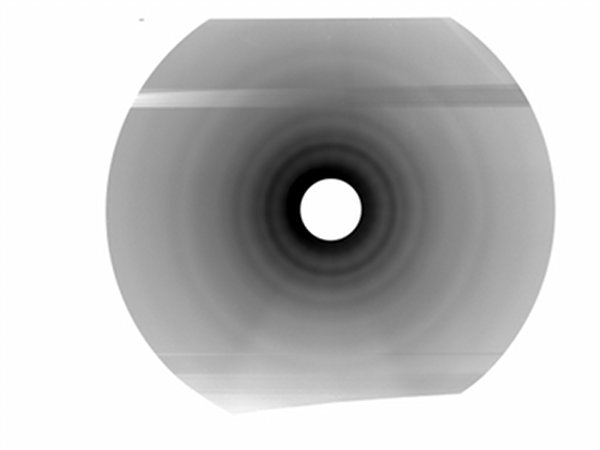
\includegraphics[width=12cm]{example}
\caption{An example of the raw data from the GED experiment.}
\label{example} 
\end{figure} 


 
% graphical user interface howto 
   \section{Description of the user interface}\label{interface} 
The graphical user interface is very easy to use. An example is given in Figure~\ref{ui} (p. \pageref{ui}) how the interface looks like. 

\begin{figure}
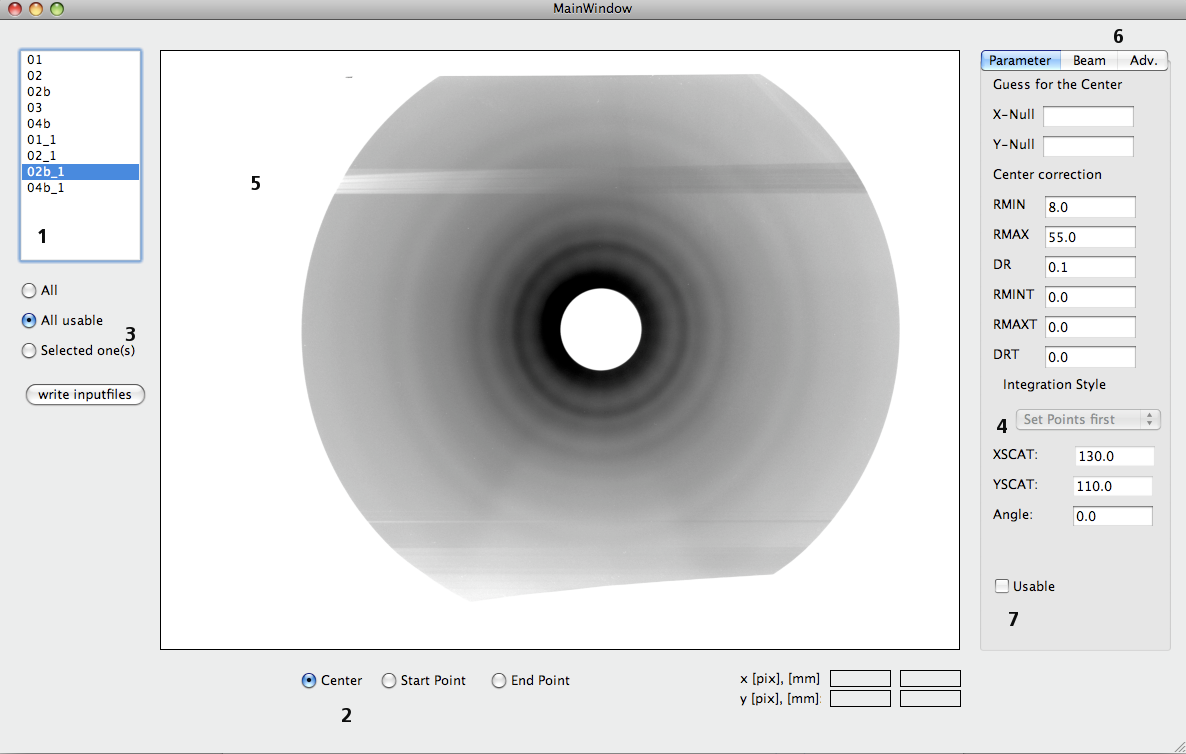
\includegraphics[width=20cm, angle=90]{ui.png}
\caption{Typical screenshot of the user interface. (1) The itemlist (listWidget), (2) Radiobuttons for selecting points, (3) Radiobuttons for selecting which input files to write out, (4) drop-down menu for selecting data reduction style, (5) main graphic, (6) tabs to set more parameters and (7) the usable checkbox. }
\label{ui} 
\end{figure} 

\subsection{Input}
The program can deal with all kind of image formats. It was tested with .tif files but should work with all other formats, as long as they are supported by Qt. \\
The the images can be opened with the OpenFile menu. \\
The following should be considered:
\begin{enumerate}
\item The program assumes that the data files (.img) are in the same directory then the image files (.tif). 
\item The pimag executable must be in the same directory then the .tif and .img files. Otherwise the data reduction (see later) will not work. 
\end{enumerate}

\subsection{Workflow}
A complete workflow is described in Figure~\ref{workflow} (p. \pageref{workflow}). The workflow describes one way to work with the program. Theoretically it is possible to go back at any point of the diagram. 

\begin{figure}
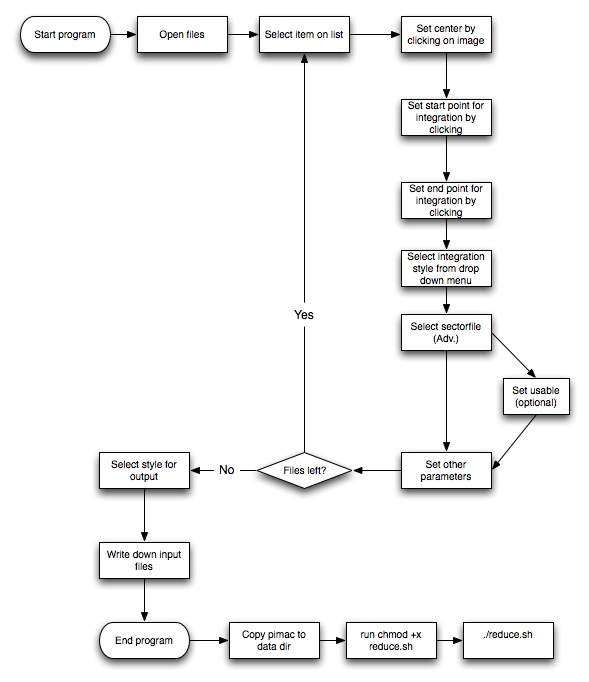
\includegraphics[width=12cm]{diagram}
\caption{Workflow of the program.The "set usable"-step is optional, depending on the way the input files are written out later. If you decide to write out input files for every image, it is not necessary to set.  }
\label{workflow} 
\end{figure} 

\subsection{Output}
The program hast tree modes to write out input files for pimag. For all images imported, for all images selected in the list or for all images flagged as usable. \\
For every image one .txt file is written out to the same directory then the image files. \\
In the end a bash-script is written do reduce.sh that can be used for data reduction. Notice that it must be executable (chmod +x) to execute it. Assuming the .tif and .img files are in /home/geduser/mydata/, the following has to be done: \\

\begin{lstlisting}
cd /home/geduser/mydata/
chmod +x reduce.sh
./reduce.sh 
\end{lstlisting}

The last command starts the data reduction. The script creates (or overrides!) the following files, assuming that \$filename was the name of the .tif file, without the .tif.  

\begin{itemize}
\item [\$filename.curv] This file is used for further processing of the data. 
\item [\$filename.plot] This file is used for plotting, a free program like xmgr \cite{xmgr} or GNUPLOT \cite{gnuplot} can be used. 
\end{itemize}





% techstuff
   \section{Technical documentation}\label{tech}
\subsection{Installation}
The program is available via a git repository \cite{git}. To get the program just clone the repository with typing in bash: 
\begin{lstlisting}
git clone git://github.com/twesterm/ged-interface.git
\end{lstlisting}
To compile the program Qt 4.5 \cite{qt} hast to be installed. There are packages available for every major Linux distribution, Mac OS X and Windows. Enter the get-interface directory and build with: 
\begin{lstlisting}
qmake
make
\end{lstlisting}
A binary GED oder GED.app (Mac OS X) is created which can be used. \\
The compile PIMAG, enter the ged-interface/pimag/ directory and run the compile script with: 
\begin{lstlisting}
./compile
\end{lstlisting}
Note that there is Intel FORTRAN compiler (ifort) \cite{ifort}  is necessary to compile pimag. A pimag binary is produced that have to be copied. 

\subsection{Program structure}
The program is written in C++ using Qt 4.5 (documentation online: \cite{qtdoc}).\\
 Data management is done via a QListWidget using GEDItem as a custom class for the Items of the list. GEDItem is inherited from QListWidgetItem. Most explanations are written as comments in the source code, nevertheless the most important custom memberfunctions and properties will be discussed in detail. \\
 
 
\subsection{The GEDItem class}
The definition of the GEDItem class read as: 
\begin{lstlisting}
class GEDItem : public QListWidgetItem
\end{lstlisting}
All inherited functions, slots, signals and properties are documented online \cite{qtdoc}.     \\
\subsubsection{Properties} 
 The (private) properties of the GEDItem class are: 
\begin{lstlisting}
private: 
      QString IPLA, IXMA, JYMA;
      QString PIXEL, XPIXFA, YPIXFA, XSCAT, YSCAT, XNULL, YNULL, RMIN, RMAX, DR, RMINT, RMAXT, DRT, TUNEXP, RADI, CADIST;
      QString WAVE, DELTAS, SEPLA, ISECT, IRECOA, IRECOA2, ANGLE, SECFI;
      bool Useable;
      QString Path, Mode;
      QString xRMAXT, yRMAXT, xAngle, yAngle;
\end{lstlisting}
There are get- and setmethods for every private property of the class named getProperty and setProperty. 
\subsubsection{float GEDItem::distance(float x1, float x2, float y1, float y2)} 
Gets two points $p_1$ and $p_2$ in $\mathbb{R}^2$ and returns the distance between the points. 

\subsubsection{float GEDItem::calcAngle(float x1, float y1, float x2, float y2, float x3, float y3)}
Gets a triangle defined by points $p_1$, $p_2$ and $p_3$ in $\mathbb{R}^2$ and returns the angle in the defined triangle at $p_1$. 

\subsubsection{QString GEDItem::writeInputFile()}
Writes out an input file for PIMAG \cite{pimag} and returns a QString with the complete filename (including path) of the written file. \\
The complete filename of the input file is the same then the selected .tif file, but with .txt instead of .tif.  The returned filename is used for a list in QMainWindow. \\

\newpage

\subsection{The QMainWindow Class} 
This class handles the main window and all of it's slots and signals with the instance ui. The definition reads as:
\begin{lstlisting}
class MainWindowClass : public QMainWindow
\end{lstlisting}
The only notable property of QMainWindow is \lstinline$ QStringList fileList $ that contains the list of all inputfiles that have been written to hard drive. 

\subsubsection{bool MainWindowClass::eventFilter( QObject $\ast$ watched, QEvent  $\ast$ event )[slot]}
Is the primary eventfilter of the program. It handles all events coming from \lstinline$ ui->picLabel$ (the picture-frame of the program). \\
Returns if the events was handled, always false (for internal reason). 

\subsubsection{bool MainWindowClass::isIn(QString name)  [slot]  } 
Returns true, if the name is already in the list of the listWidget. 

\subsubsection{ void MainWindowClass::on\_actionOpenFile\_triggered()  [slot] }
Executes if the user clicks on openfile. Handles all renaming of doubled items in the listWidget and ads the selected files to the listWidget as GEDItems. 

\subsubsection{void MainWindowClass::setValuesByMethod(QString method) }
When this function is called, it calculates the values for XSCAT, YSCAT and ANGLE and writes them to the corresponding lineEdits at the user interface.  

\subsubsection{void MainWindowClass::on\_listWidget\_ itemClicked (QListWidgetItem  $\ast$ item) [ slot ] }
Is called when the user clicks on an item at the listWidget. It sets all stored values to the lineEdit forms, sets the picture and calls  setValuesByMethod(). 

\subsection{Porting to Windows} 
In general it is possible to port \textit{GED ready} to windows. There are two main problems: \\
1.: String processing. The following memberfunctions do string manipulation and would have to be carefully modified to take the difference in file names into account: 
\begin{lstlisting}
void MainWindowClass::on_actionOpenFile_triggered()
void MainWindowClass::on_IntegratePushButton_pressed()
QString GEDItem::writeInputFile() 
\end{lstlisting}
2.: The \lstinline! void MainWindowClass::on_IntegratePushButton_pressed() ! would have to be modified to produce scripts for Microsoft Power Shell. 






   
%results
 %  \include{appendix}

\section{References} 
\bibliography{till}
\end{document}
